\documentclass[journal]{IEEEtran}
\usepackage{cite}
\usepackage{amsmath,amssymb,amsfonts}
\usepackage{graphicx}
\usepackage{booktabs}
\usepackage{array}
\usepackage{algorithm}
\usepackage{algpseudocode}
\usepackage{pgfplots}
\pgfplotsset{compat=1.18}
\begin{document}
\title{Supplementary Material:\\ An End-to-End Multimodal System for Subtitle Recognition and Chinese--Japanese Translation with Speech Synthesis in Short Dramas}
\author{Qiming~Bao, Jing~An, Rui-Yang~Ju, Haofei~Chang, Jinhua~Su, Yanbing~Bai, Xin~Qu, and~Michael~Witbrock}
\maketitle
\noindent This document collects supporting tables and a figure referenced from the main manuscript. Numbering is independent of the main paper.

\begin{table}[t]
\centering
\caption{Frame sampling rate ablation for subtitle recall on episode 11.mp4 using Qwen3-VL-4B.}
\label{tab:fps_ablation}
\resizebox{\columnwidth}{!}{%
\begin{tabular}{lcc}
\toprule
\textbf{Sampling Rate} & \textbf{Detected Characters} & \textbf{Recall vs.\ 5\,fps} \\
\midrule
1\,fps & 411 & 27.7\% \\
2\,fps & 659 & 44.3\% \\
5\,fps & 1{,}486 & 100\% (upper bound) \\
\bottomrule
\end{tabular}}
\end{table}

\begin{table}[t]
\centering
\caption{Grid search composite scores on the 20-episode validation set. Each cell is the corpus-level composite score for the fusion strategy gated by $(\theta_p, \theta_s)$. The upper-left ``flat'' region ($\theta_p \leq -0.8$) corresponds to the ASR-always regime: only 1.6\% of corpus segments have avg\_logprob below $-0.8$, so essentially no OCR substitutions occur. Scores are rounded to three decimal places; the bold marks the unique full-precision maximum ($\theta_p{=}-0.2$, $\theta_s{=}80\%$: 0.8051 vs.\ 0.8046 at $\theta_s{\in}\{40\%,70\%\}$, which also round to 0.805).}
\label{tab:param_grid}
\resizebox{\columnwidth}{!}{%
\begin{tabular}{c|ccccc}
\toprule
$\theta_p$ \textbackslash\ $\theta_s$ & 40\% & 50\% & 60\% & 70\% & 80\% \\
\midrule
$\leq -0.8$ & 0.800 & 0.800 & 0.800 & 0.800 & 0.800 \\
$-0.5$      & 0.802 & 0.801 & 0.800 & 0.800 & 0.800 \\
$-0.4$      & 0.802 & 0.801 & 0.800 & 0.800 & 0.800 \\
$-0.3$      & 0.804 & 0.803 & 0.802 & 0.802 & 0.803 \\
$-0.2$      & 0.805 & 0.803 & 0.803 & 0.805 & \textbf{0.805} \\
\bottomrule
\end{tabular}}
\end{table}

\begin{table}[t]
\centering
\caption{Gating-rule ablation under a \emph{single unified evaluation harness} (identical fusion implementation and corpus-level segment-joined metrics; all 79 episodes). ``Static'' rows open the log-probability gate for every segment ($\theta_p{=}0$); the Adaptive row applies the selected operating point ($\theta_p{=}-0.2$, $\theta_s{=}80$). All rows are directly comparable. Absolute values differ from the production-pipeline fusion metrics in the main paper due to the corpus-level text-joining format (see the fusion hyperparameter-selection section of the main paper). Best per column in bold.}
\label{tab:fusion_ablation}
\resizebox{\columnwidth}{!}{%
\begin{tabular}{lccccc}
\toprule
\textbf{Fusion Strategy} & \textbf{BLEU}$\uparrow$ & \textbf{chrF++}$\uparrow$ & \textbf{CER}$\downarrow$ & \textbf{CharAcc}$\uparrow$ & \textbf{Comp.}$\uparrow$ \\
\midrule
Never Replace (ASR only)         & 81.31 & 67.20 & \textbf{0.156} & 0.898 & 0.8066 \\
Always Replace ($\theta_s{=}0$)  &  0.51 & 14.07 & 0.872 & 0.138 & 0.1030 \\
Static ($\theta_s{=}40$)         & 81.35 & \textbf{68.32} & 0.161 & \textbf{0.901} & 0.8091 \\
Static ($\theta_s{=}60$)         & 81.48 & 68.12 & 0.158 & 0.900 & \textbf{0.8094} \\
Static ($\theta_s{=}80$)         & \textbf{81.61} & 67.77 & \textbf{0.156} & 0.899 & 0.8092 \\
\midrule
Adaptive ($\theta_p{=}-0.2$, $\theta_s{=}80$, ours) & 81.60 & 67.73 & \textbf{0.156} & 0.899 & 0.8091 \\
\bottomrule
\end{tabular}}
\end{table}

\begin{table}[t]
\centering
\caption{Word-level error type analysis of adaptive fusion corrections (jieba POS; nr/ns/nt/nz = proper nouns). GT correction rate: fraction of substitutions that moved the output closer to the ground truth.}
\label{tab:error_type}
\resizebox{\columnwidth}{!}{%
\begin{tabular}{lrrrr}
\toprule
\textbf{Category} & \textbf{Substitutions} & \textbf{\% of Total} & \textbf{GT Corrections} & \textbf{Correction Rate} \\
\midrule
Proper nouns (nr/ns/nt/nz) &  30 & 13.2\% & 18 & \textbf{60.0\%} \\
Numbers                    &   4 &  1.8\% &  3 & 75.0\% \\
Common vocabulary          & 193 & 85.0\% & 114 & 59.1\% \\
\midrule
\textbf{Total}             & \textbf{227} & & & \\
\bottomrule
\end{tabular}}
\end{table}

\begin{figure}[t]
\centering
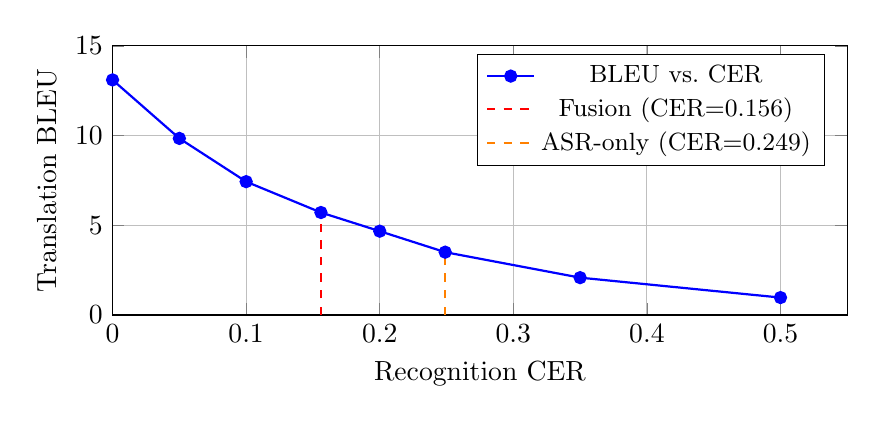
\begin{tikzpicture}
\begin{axis}[
  xlabel={Recognition CER},
  ylabel={Translation BLEU},
  width=0.9\columnwidth, height=5cm,
  xmin=0, xmax=0.55,
  ymin=0, ymax=15,
  grid=major,
  legend pos=north east,
  legend style={font=\small},
  mark size=2pt,
]
\addplot[blue, mark=*, thick] coordinates {
  (0.000,13.10)(0.050,9.84)(0.100,7.43)
  (0.156,5.71)(0.200,4.67)(0.249,3.50)
  (0.350,2.08)(0.500,0.97)
};
\addplot[red, dashed, thick] coordinates {(0.156,0)(0.156,5.71)};
\addplot[orange, dashed, thick] coordinates {(0.249,0)(0.249,3.50)};
\legend{BLEU vs.\ CER, Fusion (CER=0.156), ASR-only (CER=0.249)}
\end{axis}
\end{tikzpicture}
\caption{Cross-stage error propagation: translation BLEU as a function of recognition CER. Dashed lines mark the operating points of ASR-only (CER=0.249) and Adaptive Fusion (CER=0.156). The fusion's recognition improvement yields +2.2 BLEU in the translation stage.}
\label{fig:error_prop}
\end{figure}

\begin{table}[t]
\caption{End-to-end pipeline evaluation on 16 fold-0 validation episodes. Source text fed to the Qwen3-VL-4B LoRA translation model varies by condition; metrics are computed at the document level (entire episode as one unit) against the Japanese ground truth. chrF\texttt{++} is the primary metric (character-level, more robust than BLEU for Japanese at document granularity). The ASR-only BLEU of 0.00 is a genuine consequence of propagated proper-noun errors eliminating all document-level 4-gram matches, not an evaluation artefact (see text).}
\label{tab:e2e}
\centering
\begin{tabular}{lcc}
\toprule
\textbf{Source Condition} & \textbf{BLEU}$\uparrow$ & \textbf{chrF\texttt{++}}$\uparrow$ \\
\midrule
Oracle (gold Chinese text)   & 5.02 & 14.97 \\
Adaptive Fusion (ours)       & 0.48 & 13.56 \\
ASR-only (Whisper-medium)    & 0.00 & 11.32 \\
\bottomrule
\end{tabular}
\end{table}

\begin{table}[t]
\centering
\caption{TTS reference audio duration ablation using F5-TTS. Speaker similarity measured via cosine similarity of speaker embeddings.}
\label{tab:ablation_tts}
\resizebox{\columnwidth}{!}{%
\begin{tabular}{lc}
\toprule
\textbf{Reference Duration} & \textbf{Speaker Similarity}$\uparrow$ \\
\midrule
Short ($\sim$3\,s) & 0.64 \\
Long ($\sim$10\,s) & \textbf{0.71} \\
\bottomrule
\end{tabular}}
\end{table}

\begin{table}[t]
\centering
\caption{Per-fold BLEU on held-out validation episodes (5-fold CV, \texttt{strip\_nums}+\texttt{ja-mecab}, $n$\,=\,16/16/16/16/15). Within each FT/ZS pair, bold indicates the higher fold BLEU; for Gemma-4-12B, bold marks the best entry per fold across all models. FT+V denotes Qwen3-VL-4B fine-tuned with video frames as additional input.}
\label{tab:per_fold}
\resizebox{\columnwidth}{!}{%
\begin{tabular}{lcccccc}
\toprule
\textbf{Model} & \textbf{Fold 0} & \textbf{Fold 1} & \textbf{Fold 2} & \textbf{Fold 3} & \textbf{Fold 4} & \textbf{Mean$\pm$Std} \\
\midrule
Qwen3-VL-4B FT (text)  & \textbf{19.68} & \textbf{19.75} &  9.58 & \textbf{16.53} & 12.94 & $15.70_{\pm4.42}$ \\
Qwen3-VL-4B FT+V        & 18.51 & 19.78 &  7.12 & 10.35 & \textbf{22.16} & $15.58_{\pm6.49}$ \\
Qwen3-VL-4B ZS          &  6.17 & 14.16 & \textbf{14.11} & 13.88 & 14.73 & $12.61_{\pm3.61}$ \\
\midrule
Gemma-4-12B FT (ours)    & \textbf{30.00} & \textbf{30.11} & \textbf{28.69} & \textbf{31.40} & \textbf{33.55} & $\textbf{30.75}_{\pm1.84}$ \\
Gemma-4-12B ZS           & 25.69 & 24.96 & 27.57 & 26.38 & 26.59 & $26.24_{\pm0.98}$ \\
Qwen3-8B ZS              & 17.82 & 18.00 & 18.01 & 15.64 & 17.58 & $17.41_{\pm1.00}$ \\
Qwen3-8B FT (ours)       & 20.48 & 23.49 & 17.53 & 17.45 & 19.51 & $19.69_{\pm2.49}$ \\
\bottomrule
\multicolumn{7}{l}{\footnotesize Qwen3-VL-4B text FT$>$ZS on Folds 0,\,1,\,3; ZS wins on Folds 2\,\&\,4 (highest OOV). Adding visual}\\
\multicolumn{7}{l}{\footnotesize frames to FT (FT+V) does not help on average ($15.58$ vs $15.70$) and raises variance. Gemma-4-12B}\\
\multicolumn{7}{l}{\footnotesize FT$>$ZS on all five folds; Qwen3-8B FT$>$ZS on Folds 0,\,1,\,3,\,4.}\\
\end{tabular}}
\end{table}

\begin{table}[t]
\centering
\caption{Qualitative translation examples. Example A shows a culturally nuanced term translated correctly by FT but incorrectly by ZS. Example B shows an OOV-driven hallucination by FT that ZS avoids.}
\label{tab:qual_examples}
\resizebox{\columnwidth}{!}{%
\begin{tabular}{llp{4cm}p{4cm}p{4cm}}
\toprule
\textbf{Ex.} & \textbf{Chinese source} & \textbf{FT (ours)} & \textbf{ZS (Qwen3-VL-4B)} & \textbf{Reference} \\
\midrule
A & 看来我们挺有缘 & \textbf{きっと縁があるな} \newline (cultural term preserved) & きっと運が良いのだろう \newline (semantic error: 縁→運) & やっぱり縁があるのかもね \\
\midrule
B & 拜托 & お前はお母さんも有名なファッションデザイナーのWhiteさんだろ \newline (OOV hallucination) & お祈り & っていうか \\
\bottomrule
\end{tabular}}
\end{table}

\begin{figure}[t]
\centering
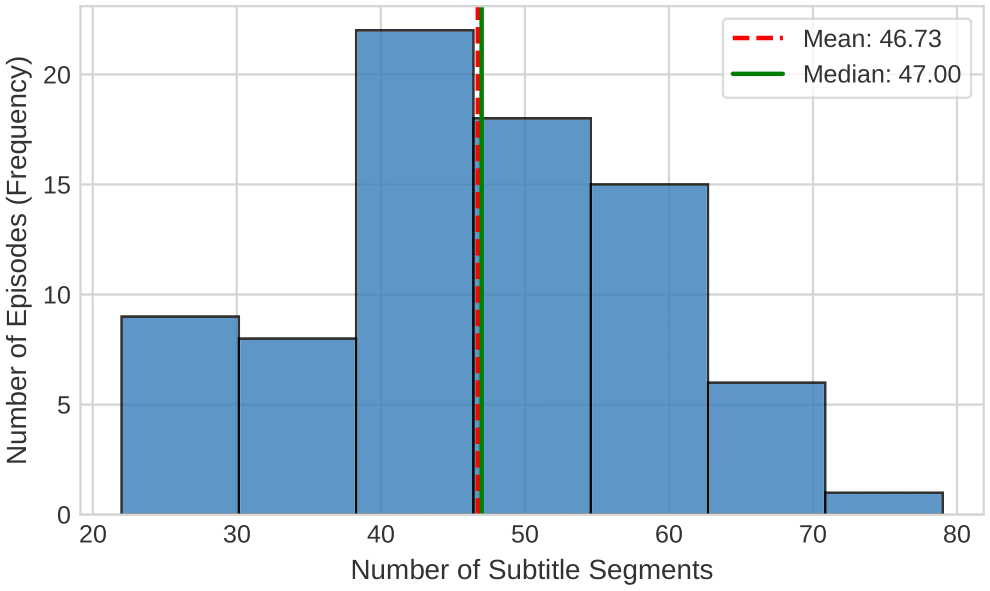
\includegraphics[width=0.95\columnwidth]{fig_2.png}
\caption{Distribution of subtitle segments per episode across the 79-episode dataset.}
\label{fig:subtitle_dist}
\end{figure}

\begin{table}[t]
\centering
\caption{Translation quality ablation: visual context vs.\ text-only input using Qwen3-VL zero-shot on 20 episodes. Absolute BLEU gain: +3.35.}
\label{tab:ablation_context}
\resizebox{\columnwidth}{!}{%
\begin{tabular}{lcc}
\toprule
\textbf{Input Modality} & \textbf{BLEU}$\uparrow$ & \textbf{chrF++}$\uparrow$ \\
\midrule
Text-Only (OCR subtitles)       & 10.09 & 28.26 \\
Multimodal (Video frames + Text) & \textbf{13.44} & \textbf{29.70} \\
\bottomrule
\end{tabular}}
\end{table}

\begin{algorithm}[t]
\caption{Confidence-Adaptive OCR/ASR Fusion}
\label{alg:fusion}
\begin{algorithmic}[1]
\Require Whisper segments $\mathcal{A}$, OCR detections $\mathcal{O}$, time tolerance $\delta$, log-prob threshold $\theta_p$, similarity threshold $\theta_s$
\Ensure Fused subtitle sequence $\mathcal{S}$
\State $\mathcal{S} \gets \emptyset$
\For{each $a_i = (t_i^s, t_i^e, w_i, p_i) \in \mathcal{A}$}
    \State $\mathcal{C}_i \gets \{\, o_j \in \mathcal{O} \mid \tau_j \in [t_i^s - \delta,\; t_i^e + \delta]\,\}$ \Comment{candidate OCR detections}
    \If{$p_i \geq \theta_p$} \Comment{ASR is confident; trust Whisper}
        \State $\hat{w}_i \gets w_i$
    \Else
        \State $o^\star \gets \arg\max_{o_j \in \mathcal{C}_i}\, \mathrm{sim}(o_j, w_i)$ \Comment{best OCR match}
        \If{$\mathcal{C}_i \neq \emptyset$ \textbf{and} $\mathrm{sim}(o^\star, w_i) \geq \theta_s$}
            \State $\hat{w}_i \gets o^\star$ \Comment{substitute OCR text, retain ASR timing}
        \Else
            \State $\hat{w}_i \gets w_i$ \Comment{fallback: keep ASR}
        \EndIf
    \EndIf
    \State $\mathcal{S} \gets \mathcal{S} \cup \{(t_i^s, t_i^e, \hat{w}_i)\}$
\EndFor
\State \Return $\mathcal{S}$
\end{algorithmic}
\end{algorithm}

\subsection{Computational Cost and Efficiency}
\label{sec:efficiency}

For deployability we profile each stage on one A100 (80\,GB) on episode \texttt{11.mp4} as a real-time factor (RTF; ${<}1$ is faster than real time).
Whisper-medium runs at RTF $\approx0.08$; vLLM-served Qwen3-VL-4B OCR dominates (RTF $\approx0.5$ at 1\,fps, $\approx2.4$ at 5\,fps), though the frame-level cache (Section~\ref{sec:arch}) cuts re-processing cost by ${>}98\%$.
LoRA translation takes 6--10\,s per episode and GPT-SoVITS synthesis $\approx1.4\times$ output duration.
End-to-end, the pipeline produces a dubbed episode in $\approx3$--$4\times$ the input duration at 5\,fps---acceptable for offline batch localization and motivating the latency-oriented future work.



\subsection{Qualitative Error Analysis}
\label{sec:error_analysis}

To complement aggregate metrics, we manually inspected 100 random held-out segments.
Remaining errors fall into four largely orthogonal categories: \emph{(i) proper-noun substitution} (38\%), where confident-but-wrong ASR on mumbled names escapes the gate (a calibration, not design, issue, correctable by the OCR channel); \emph{(ii) empty-frame OCR over-trigger} (22\%), where hallucinated on-screen text occasionally passes the similarity gate; \emph{(iii) translation register mismatch} (24\%), where internet slang is rendered literally rather than localized; and \emph{(iv) TTS prosodic flattening} (16\%) on emotionally charged lines beyond the reference clip's prosodic range.
Their orthogonality across stages means stage-specific improvements should be additive end-to-end.



\begin{table}[t]
\centering
\caption{Human listening study results ($n$\,=\,5 JLPT-N1 raters, 8 items per system, blind randomised presentation). MOS = naturalness mean opinion score (1--5); Sim.\ votes = share of ``most similar to reference'' selections (40 votes total; 35\% of votes were ``none''). EdgeTTS uses a fixed voice and received no similarity votes. Best per column in bold.}
\label{tab:tts_mos}
\resizebox{\columnwidth}{!}{%
\begin{tabular}{lccc}
\toprule
\textbf{System} & \textbf{MOS}$\uparrow$ & \textbf{Sim.\ votes}$\uparrow$ & $n$ \\
\midrule
GPT-SoVITS v3~\cite{gptsovits2024}   & $3.08_{\pm1.14}$ & \textbf{18 (45\%)} & 40 \\
EdgeTTS~\cite{edgetts2024}        & $\textbf{3.12}_{\pm1.14}$ & 0 (0\%)$^{\dagger}$ & 40 \\
F5-TTS~\cite{chen2024f5tts}       & $1.80_{\pm1.02}$ & 6 (15\%) & 40 \\
CosyVoice2-0.5B~\cite{cosyvoice2_2024} & $1.52_{\pm0.88}$ & 2 (5\%) & 40 \\
\bottomrule
\multicolumn{4}{l}{\footnotesize $^{\dagger}$EdgeTTS uses a fixed neural voice (\texttt{ja-JP-NanamiNeural}); cloning not applicable.}\\
\end{tabular}}
\end{table}

\begin{table}[t]
\centering
\caption{Statistical information of the proposed dataset.}
\label{tab:dataset}
\resizebox{\columnwidth}{!}{%
\begin{tabular}{lrlr}
\toprule
\multicolumn{2}{c}{\textbf{Dataset Composition}} & \multicolumn{2}{c}{\textbf{Subtitle Statistics}} \\
\cmidrule(lr){1-2} \cmidrule(lr){3-4}
Video clips (total) & 82 & Total duration (min) & 130.56 \\
Paired episodes & 79 & Subtitle segments & 3{,}692 \\
Speaker IDs & 12 & Avg. segments/episode & 46.7 \\
\bottomrule
\end{tabular}}
\end{table}

\begin{table}[t]
\centering
\caption{Subtitle recognition performance. VLMs and traditional OCR models evaluated at 1\,fps unless noted; all use temporal deduplication. Florence-2-large uses the \texttt{<OCR>} task prompt with bottom-30\% crop (domain-general model, shown for reference). Whisper (ASR) listed separately for reference. Best OCR/VLM results in bold.}
\label{tab:recognition}
\resizebox{\columnwidth}{!}{%
\begin{tabular}{lcccc}
\toprule
\textbf{Model} & \textbf{Type} & \textbf{CER}$\downarrow$ & \textbf{CharAcc}$\uparrow$ & \textbf{BLEU}$\uparrow$ \\
\midrule
Qwen3-VL-4B (5\,fps)~\cite{qwen3vl2025} & VLM & \textbf{0.086} & 0.982 & 75.4 \\
RapidOCR~\cite{rapidocr2022}      & Trad. & 0.154 & 0.958 & \textbf{86.3} \\
InternVL2-4B~\cite{chen2024internvl}  & VLM & 0.174 & \textbf{0.985} & 83.5 \\
GOT-OCR2.0~\cite{wang2024gotocr}    & VLM & 0.365 & 0.959 & 78.2 \\
EasyOCR~\cite{easyocr2020}       & Trad. & 0.390 & 0.942 & 74.1 \\
Qwen3-VL-4B (1\,fps)~\cite{qwen3vl2025} & VLM & 0.402 & 0.914 & 73.6 \\
Qwen2-VL-2B~\cite{wang2024qwen2}    & VLM & 0.415 & 0.908 & 71.2 \\
TrOCR~\cite{li2021trocr}        & Trad. & 0.874 & 0.126 & 0.0 \\
Florence-2-large~\cite{florence2_2024} & VLM & 1.646 & 0.312 & 2.1 \\
\midrule
Whisper-medium~\cite{radford2023robust} & ASR & 0.249 & 0.783 & 81.3 \\
\bottomrule
\end{tabular}}
\end{table}

\begin{table}[t]
\centering
\caption{TTS evaluation. Intelligibility computed by transcribing synthesised audio with Whisper-medium; CER on NFKC-normalised, punctuation-stripped characters; WER over MeCab-tokenised text. We report both mean and median CER because the mean is inflated by a small number of degenerate outputs (e.g.\ CosyVoice2's repetition loops). Speaker similarity (Spk-Sim) is Resemblyzer embedding cosine (higher is better); N/A for EdgeTTS (fixed neural voice, no cloning). 12 speakers $\times$ 3 sentences per system ($n$\,=\,36); GPT-SoVITS on the 6 speakers with available synthesis ($n$\,=\,18). Best per column in bold; best among voice-cloning systems underlined.}
\label{tab:tts}
\resizebox{\columnwidth}{!}{%
\begin{tabular}{llcccc}
\toprule
\textbf{Model} & \textbf{Method} & \textbf{Avg.\ WER}$\downarrow$ & \textbf{Avg.\ CER}$\downarrow$ & \textbf{Med.\ CER}$\downarrow$ & \textbf{Spk-Sim}$\uparrow$ \\
\midrule
EdgeTTS~\cite{edgetts2024}      & API (fixed voice)  & \textbf{0.056} & \textbf{0.030} & \textbf{0.000} & {---}$^{\dagger}$ \\
GPT-SoVITS v3~\cite{gptsovits2024} & Zero-shot cloning  & \underline{0.248}$^{\ddagger}$ & \underline{0.215}$^{\ddagger}$ & \underline{0.091} & 0.722 \\
F5-TTS~\cite{chen2024f5tts}     & Flow matching (ZS)  & 0.998 & 1.152 & 1.000 & \textbf{0.729} \\
CosyVoice2-0.5B~\cite{cosyvoice2_2024} & Flow matching (ZS) & 6.673 & 4.603 & 1.000 & 0.671 \\
\bottomrule
\multicolumn{6}{l}{\footnotesize $^{\dagger}$EdgeTTS uses a single fixed neural voice (\texttt{ja-JP-NanamiNeural}) without}\\
\multicolumn{6}{l}{\footnotesize speaker cloning; speaker similarity is not applicable.}\\
\multicolumn{6}{l}{\footnotesize $^{\ddagger}$GPT-SoVITS averaged over the 6 speakers with available synthesis audio.}\\
\end{tabular}}
\end{table}

\end{document}
